\subsection{Stability Analysis of the Equilibrium}



Question 2 presents an unstable state in which the population of organism 2 ($N_2$) dominates and reduces the population of organism 1($N_1$) to local extinction. The proposed intervention involved reducing the populations of both $N_1$ and $N_2$ by a constant factor $\rho \in (0,1)$ The question is, is this intervention effective and if so, is there a range of value of $\rho$ in which the intervention is effective? 

More formally the state of the system is represented by a vector 
$$ \textbf{N} = \begin{bmatrix}N_1 \\ N_2\end{bmatrix}$$
The system is an an region of the system that moves towards an equilibrium where $N_1=0$. The question is then: is there some scalar value $\rho$ which results in the system moving towards an equilibirum where $N_1, N_2 > 0$

The result of the reduction reduction by rho is a vector $\textbf{N'}$

$$ \textbf{N'} = \begin{bmatrix}N_1' \\ N_2'\end{bmatrix}$$

Since $\textbf{N}$ is multiplied by a scalar, $\textbf{N'}$ will have the same direction as $\textbf{N}$, but a smaller magnitude. 

From the initial wording of the question we know that $N1$ goes to 0. In order for an intervention to be successful the scaled $\textbf{N'}$ must fall within a region such that the evolution will not cause the population of  $N_1$ to go to 0. Fig \ref{fig:phase_flow} depicts this process. 

This is not possible for the following reason. The derivative $\dot{N_1} $ constantly decreases going from positive to negative as it crossed the $N_1$ nullcline. An intervention can change the magnitude of $\textbf{N}$ but not the direction so the resulting intervention will pull $\textbf{N}$ the same distance or closer towards $N_1 = 0$. As a result no intervention and no value of rho can prevent the population of species 1 from collapsing. 


\begin{figure}[h]
  \centering
  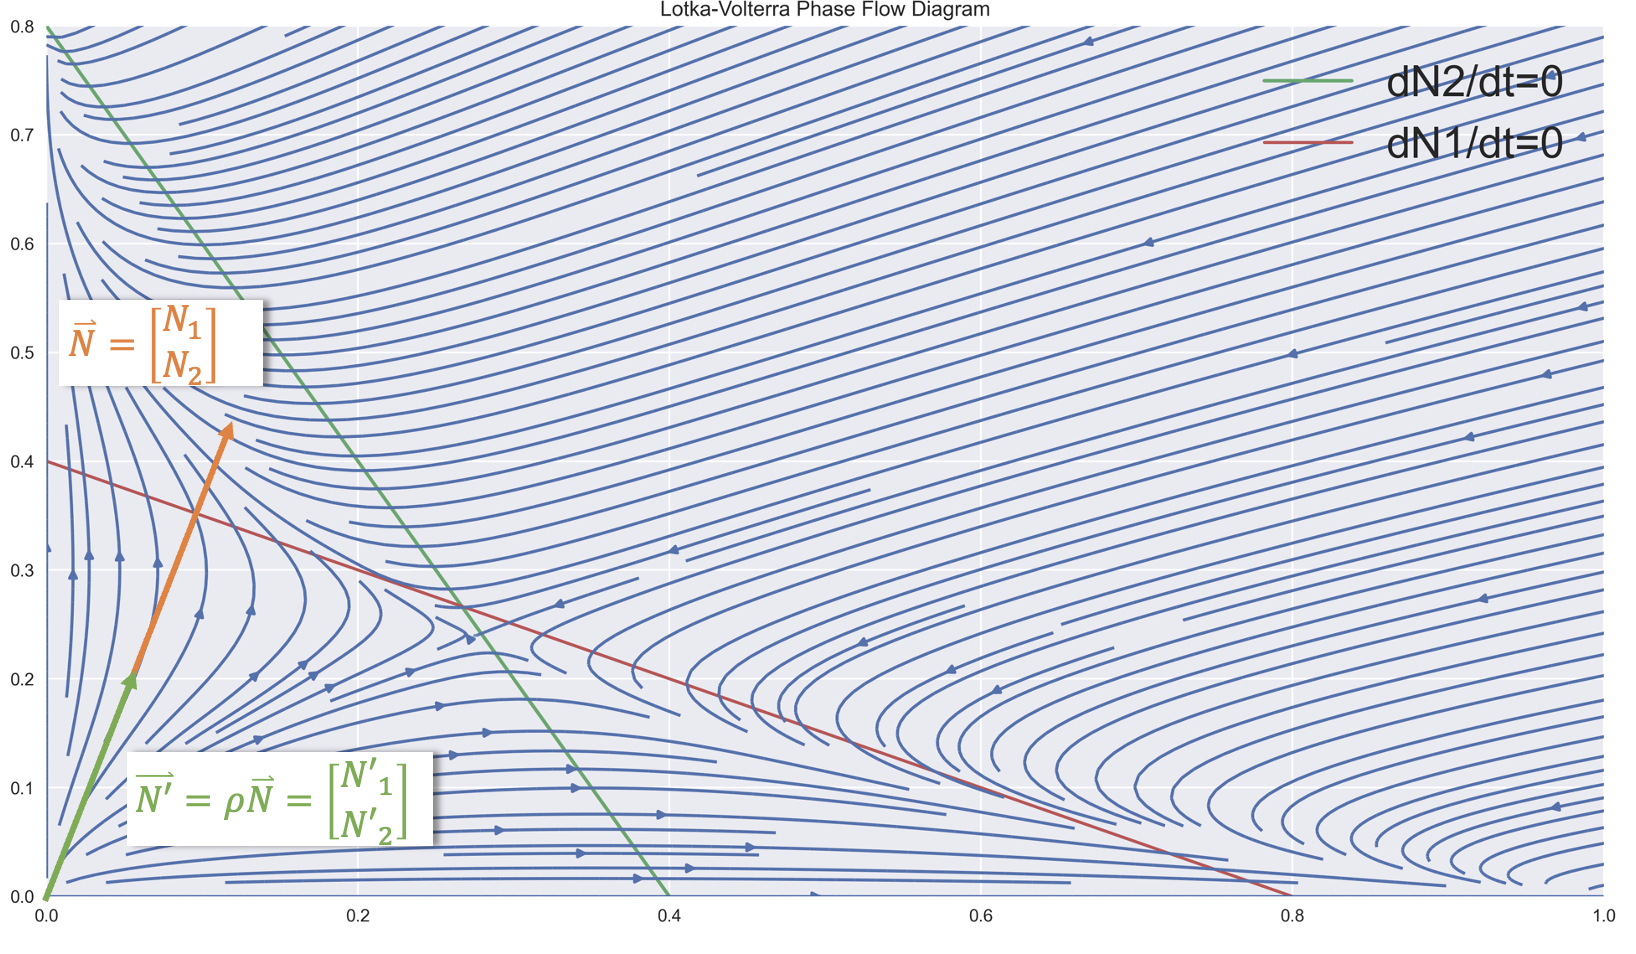
\includegraphics[width = \textwidth]{fig/graph_004.png}
  \caption {A phase flow diagram of the Lotka Volterra Model, the state of the system at any time is specified by a vector $\vec{N}$, the reduction by rho then corresponds to multiplying this vector by a scalar quantity $\rho$ to a resulting vector $\vec{N'}$}. 
  \label{fig:phase_flow}
\end{figure}


\begin{figure}[h]
  \centering
  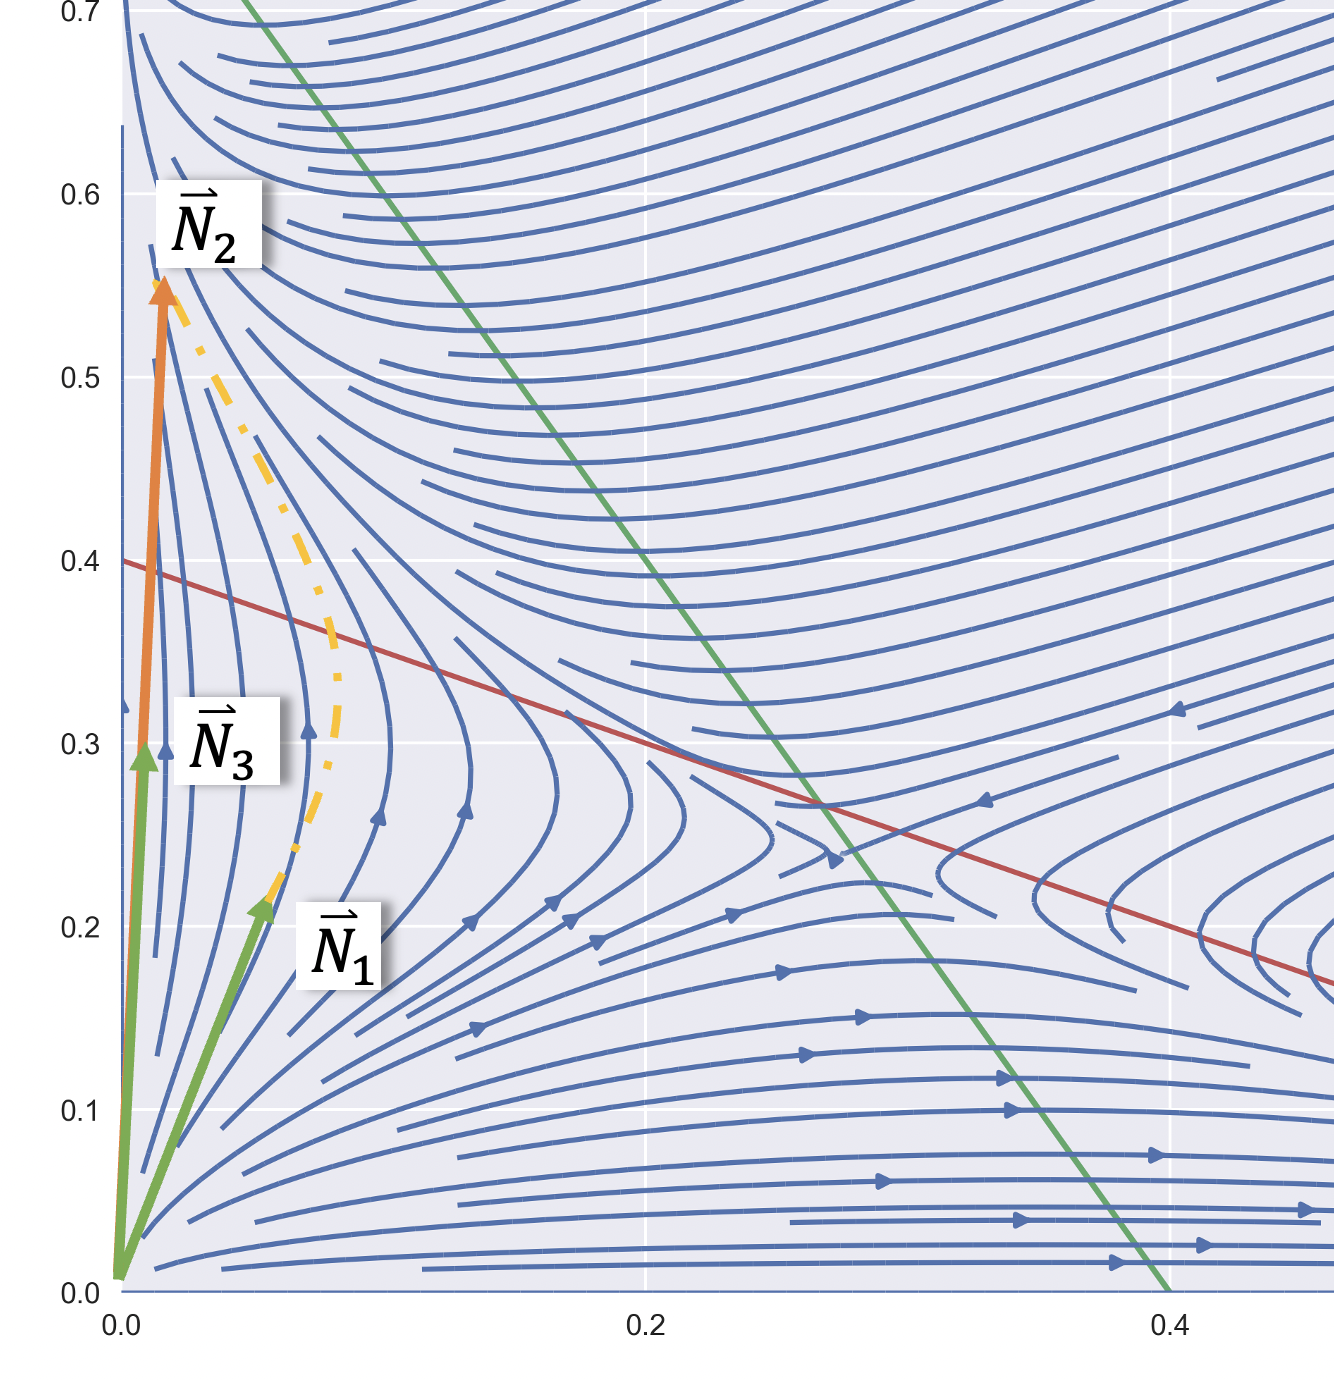
\includegraphics[width = \textwidth]{fig/graph_005.png}
  \caption {The result of an intervention by reducing the population by $\rho$. The state begins at $\vec{N_1}$ and evolves forward in time. The system evolves in time forward crossing the nullcline to into the region on the top right.}. 
  \label{fig:phase_flow_intervention}
\end{figure}

